\documentclass[]{article}

\usepackage{tabu}
\usepackage{amsfonts}
\usepackage{amsmath}
\usepackage{graphicx}

\setlength{\tabcolsep}{12pt}
\renewcommand{\arraystretch}{2}

%opening
\title{CSE 306\_Assignment1 \\
4-Bit Arithmetic and Logic Unit}
\author{ \\ Student ID : 1505097-1505102}





\begin{document}
\maketitle

\vspace{5cm}

\begin{figure}[h!]
    \centering
    
\includegraphics[width = 0.3\textwidth]{logo.png}
    \label{fig:bl}
\end{figure}
\begin{center}
   \Large{ Department of Computer Science and Engineering
 \\ Bangladesh University of Engineering and Technology
 \\ (BUET) \\
Dhaka 1000 \\}

\end{center}



\newpage
	%--------------------------------------------------------arithmetic
	\section{Design of Arithmetic Unit}
	
	\textbf{Truth Table : Arithmetic Operations}
	\begin{center}
		\begin{tabular}{ |c|c|c|c|c|c| } 
			\hline
			$cs_2$ & $cs_1$ & $cs_0(c_{in})$ & Arithmetic Operation & $x_i$ & $y_i$  \\
			\hline
			
			\hline
			0 & 0 & 0 & Subtract with borrow & $A_i$ & $\overline{B_i}$ \\
			\hline

			\hline
			0 & 0 & 1 & Subtract & $A_i$ &$\overline{B_i}$\\
			\hline
			
			\hline
			0 & 1 & 0 & Decrement A & $A_i$ & $1$ \\
			\hline
			
			\hline
			0 & 1 & 1 & Transfer A & $A_i$ & $1$ \\
			\hline
			
		\end{tabular}
	\end{center}
	
	
	\textit{Subtract : } \newline
	$=A-B$ \newline
	$=(A+\overline{B}+1)$ \newline
	\newline
	
	
	\textit{Subtract with borrow explanation:}\newline
	$=A-B-1$ \newline
	$=(A+\overline{B}+1)-1$ \newline
	$=A+\overline{B}$ \newline
	\newline
	
	\textit{Decrement A :}\newline
	$=A-1$ \newline
	$=A+(all 1) + 0 $ \newline
    \newline
	
	\textit{Transfer A :}\newline
	$=A$ \newline
	$=A+(all 1) + 1 $ \newline
	\newline
	
	
	So,
		$Y_i=\overline{CS_1}.\overline{B_i}+CS_1 = \overline{(CS_1+B_i)}+CS_1$
	\begin{figure}[h!]
		\centering
		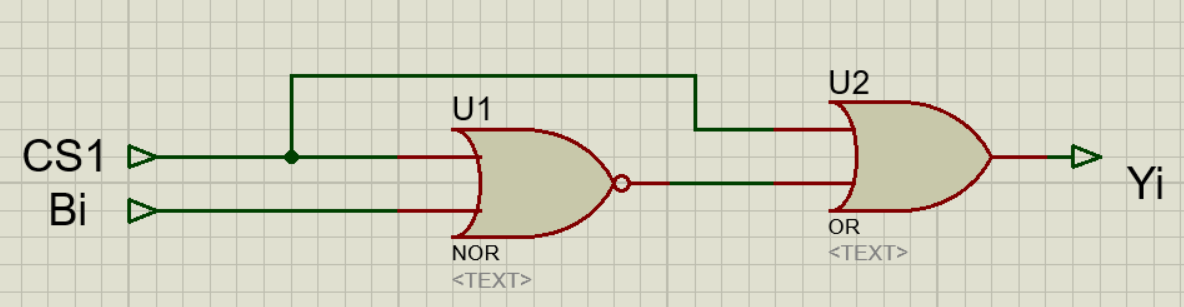
\includegraphics[width = 0.5\textwidth]{Yi.PNG}
		\caption{Design of Yi}
		\label{fig:ckt1}
		
	\end{figure}
	%--------------------------------------------------------arithmetic
	
	%--------------------------------------------------------logic
	\section{Design of Logic Unit}
	\textbf{Truth Table : Logical Operations}
		\begin{center}
		\begin{tabular}{ |c|c|c|c|c|c|c| } 
			\hline
			$cs_2$ & $cs_1$ & $cs_0(c_{in})$ & $x_i$ & $y_i$ & $F_i=X_i \oplus Y_i$ & Operation \\
			\hline
			
			\hline
			1 & 0 & 0 & $A_i+\overline{B_i}$ & $B_i$ & $A_i.B_i$ & AND \\
			\hline
			
			\hline
			1 & 0 & 1 & $A_i+\overline{B_i}$ & $B_i$ & $A_i.B_i$ & AND \\
			\hline
			
			\hline
			1 & 1 & 0 & $\overline{A_i}$ & $0$ & $\overline{A_i}$ & Complement A \\
			\hline
			
			\hline
			1 & 1 & 1 & $\overline{A_i}$ & $0$ & $\overline{A_i}$ & Complement A\\
			\hline
		\end{tabular}
	\end{center}

	\textbf{Explanation:}\newline
	we can't modify $Y_i$ because that would change the arithmetic operations
	and neither can omit $A_i$ in any input, So we change $X_i$,\newline
	Let,

	$X_i=A_i+K_i$ \newline
	$F_i=X_i \oplus Y_i$ \newline
	$F_i=X_i \oplus 0$ \newline
	$F_i=X_i$ \newline
	$F_i=A_i+K_i$\newline
	
	But the desired output is $A_i+B_i$. So putting $K_i=B_i$ \newline
	$F_i=X_i \oplus Y_i$\newline
	$F_i=(A_i \oplus K_i) \oplus \overline{B_i}$\newline
	$F_i=(A_i \oplus K_i)B_i + \overline{(A_i \oplus K_i)} .\overline{B_i}$\newline
	$F_i=A_iB_i + K_iB_i + \overline{A_i}.\overline{K_i}.\overline{B_i}$ \newline Here our desired operation is $A_iB_i$ \newline
	So, $A_iB_i + K_iB_i + \overline{A_i}.\overline{K_i}.\overline{B_i} = A_iB_i$\newline if $K_i=\overline{B_i}$	Then $F_i=A_iB_i$\newline
	So we need $K_i=B_i$ when we will do OR operation and $K_i=\overline{B_i}$ for AND operation.
	
	\begin{center}
		\begin{tabular}{|c|c|c|c|}
			\hline
			$cs_2$ & $cs_1$ & $cs_0$ & $B$ \\
			\hline
			
			\hline
			$1$ & $0$ & $0$ & $\overline{B_i}$ \\
			\hline
			
			\hline
			$1$ & $0$ & $1$ & $\overline{B_i}$ \\
			\hline
			
			\hline
			$1$ & $1$ & $0$ & $0$ \\
			\hline
			
			\hline
			$1$ & $1$ & $1$ & $0$ \\
			\hline
		\end{tabular}
	\end{center}
	So from the truth table we can derive, \newline
	$X_i=A_i+CS_2.\overline{CS_1}.\overline{B_i}=A_i+CS_2\overline{(CS_1+B_i)} $\newline
	
	\begin{figure}[h!]
		\centering
		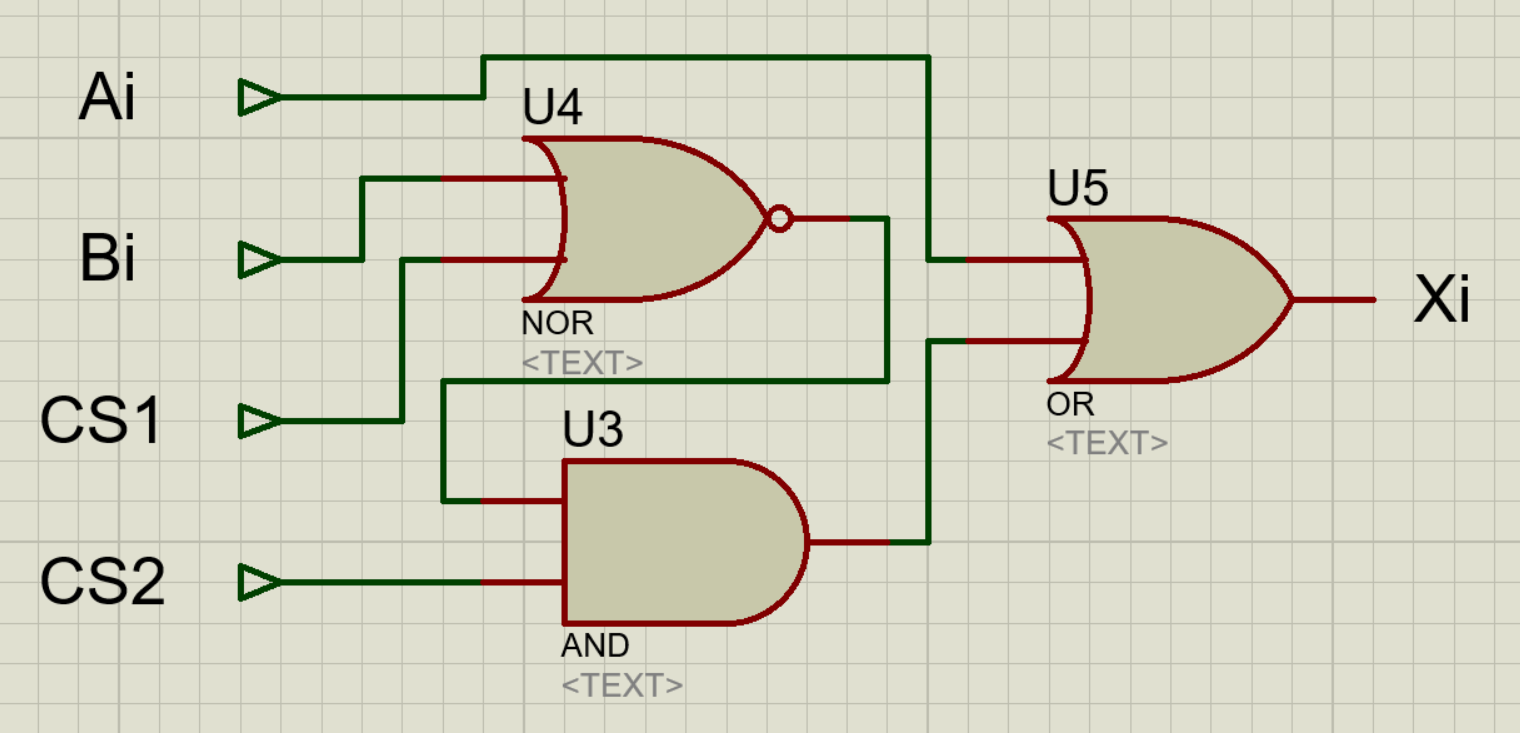
\includegraphics[width = 0.5\textwidth]{Xi.PNG}
		\caption{Design of $X_i$ \newline
		}
		\label{fig:ckt2}
		
	\end{figure}

	\section{Final Diagram}
	$X_i=A_i+CS_2\overline{(CS_1+B_i)}$
	\newline
	\newline
    $Y_i = \overline{(CS_1+B_i)}+CS_1$
    \begin{figure}[h!]
		\centering
		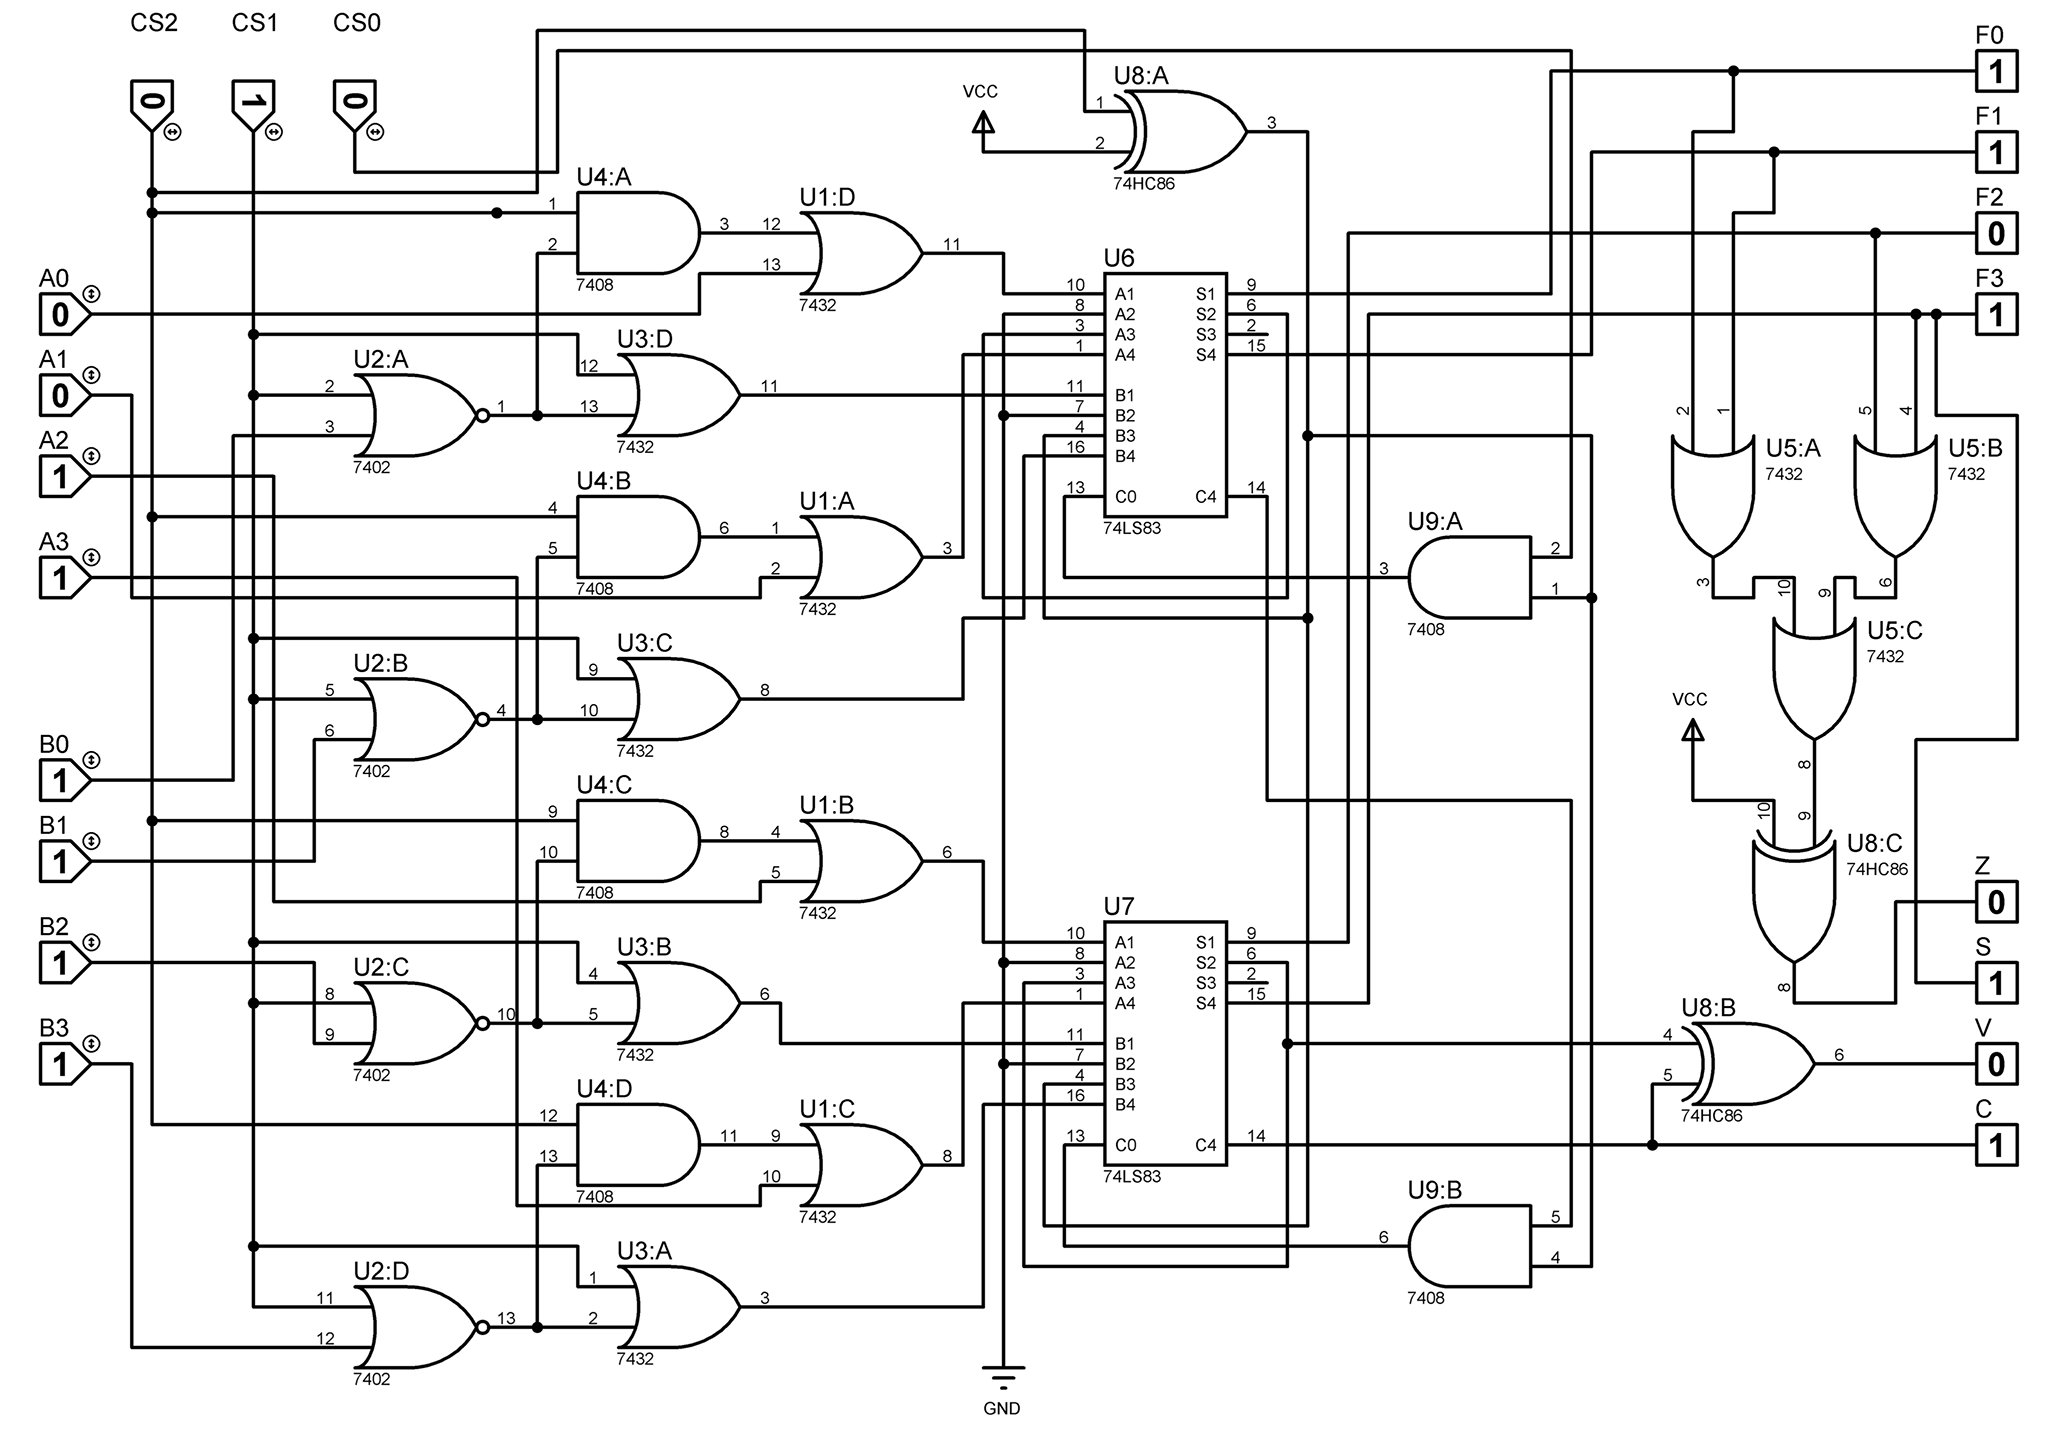
\includegraphics[width = 1\textwidth]{Total.png}
		\caption{Diagram of ALU \newline
		}
		\label{fig:ckt3}
		
	\end{figure}
	
	
	%--------------------------------------------------------logic	
\end{document}
